\documentclass[12pt, a4paper]{book}
\usepackage[width=4.375in, height=7.0in, top=1.0in, papersize={5.5in,8.5in}]{geometry}
\usepackage{indentfirst}
\usepackage[utf8]{inputenc}
\usepackage[T1]{fontenc}
\usepackage{ebgaramond}
\usepackage{imakeidx}

\usepackage{fancyhdr}
\usepackage{titlesec}
\usepackage{poemscol}
\usepackage{graphicx}

\pagestyle{fancy}
\fancyhf{}
\rhead{\thepage}
\lhead{\leftmark}
\title{
\setlength{\fboxsep}{3pt}%
\setlength{\fboxrule}{3pt}%
\fbox{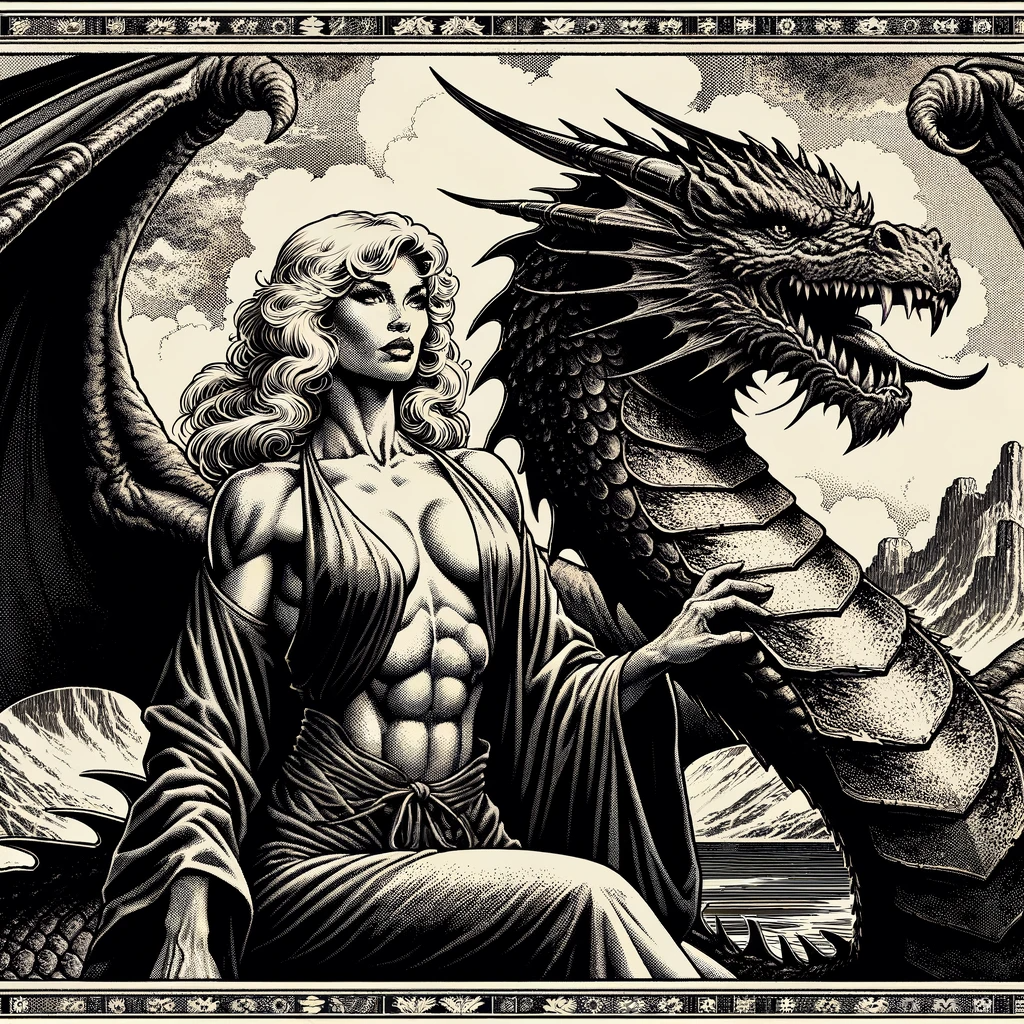
\includegraphics[width=0.5\textwidth]{front cover 2.png}}~\\[1cm]
Platebreaker\\-\\A Pulp Fantasy Collection
}
\author{Andrew Lovick}
\date{}

\makeindex

\begin{document}
\pagenumbering{gobble}
\maketitle
\clearpage
\tableofcontents	
\printindex
\begin{center}
\setlength{\fboxsep}{3pt}%
\setlength{\fboxrule}{3pt}%
\fbox{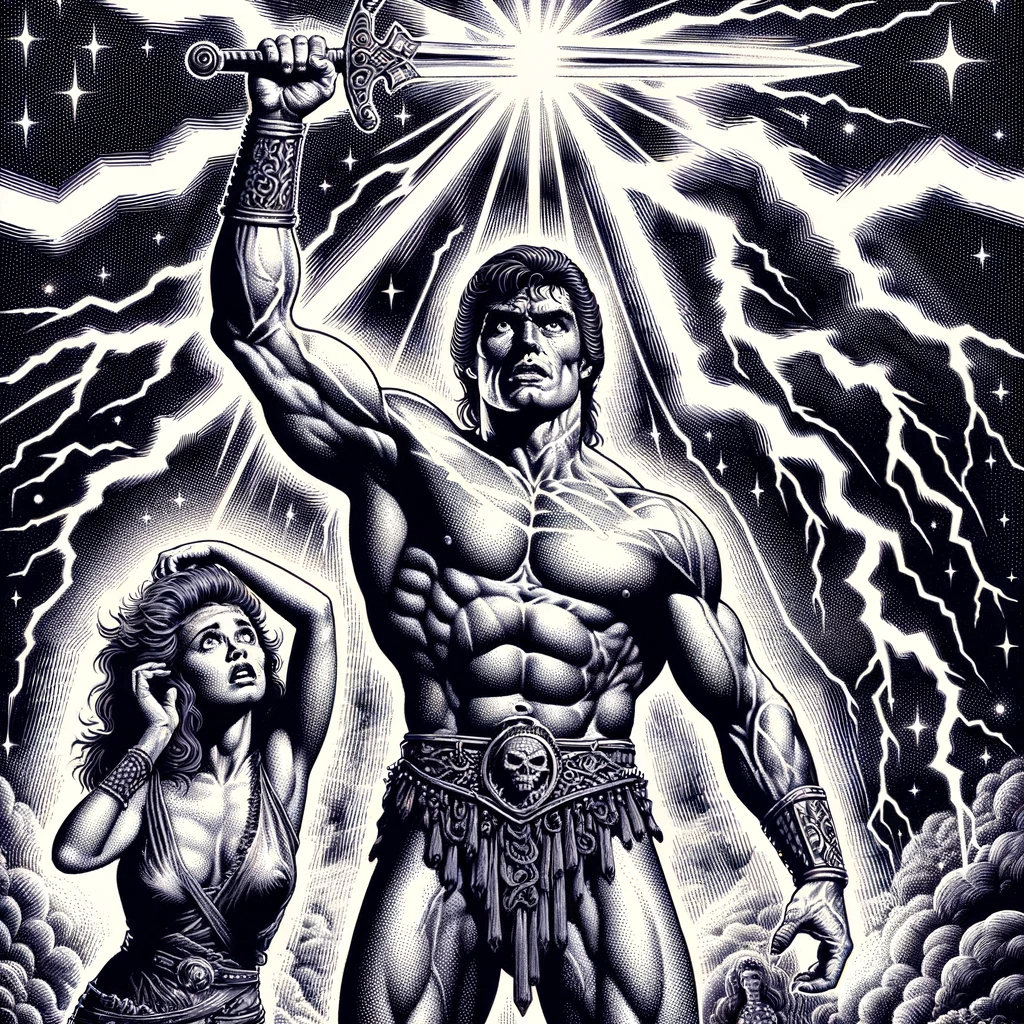
\includegraphics[width=0.5\textwidth]{front cover 3.png}}~\\[1cm]
\end{center}
\clearpage
\pagenumbering{arabic}
\part*{
\setlength{\fboxsep}{3pt}%
\setlength{\fboxrule}{3pt}%
\fbox{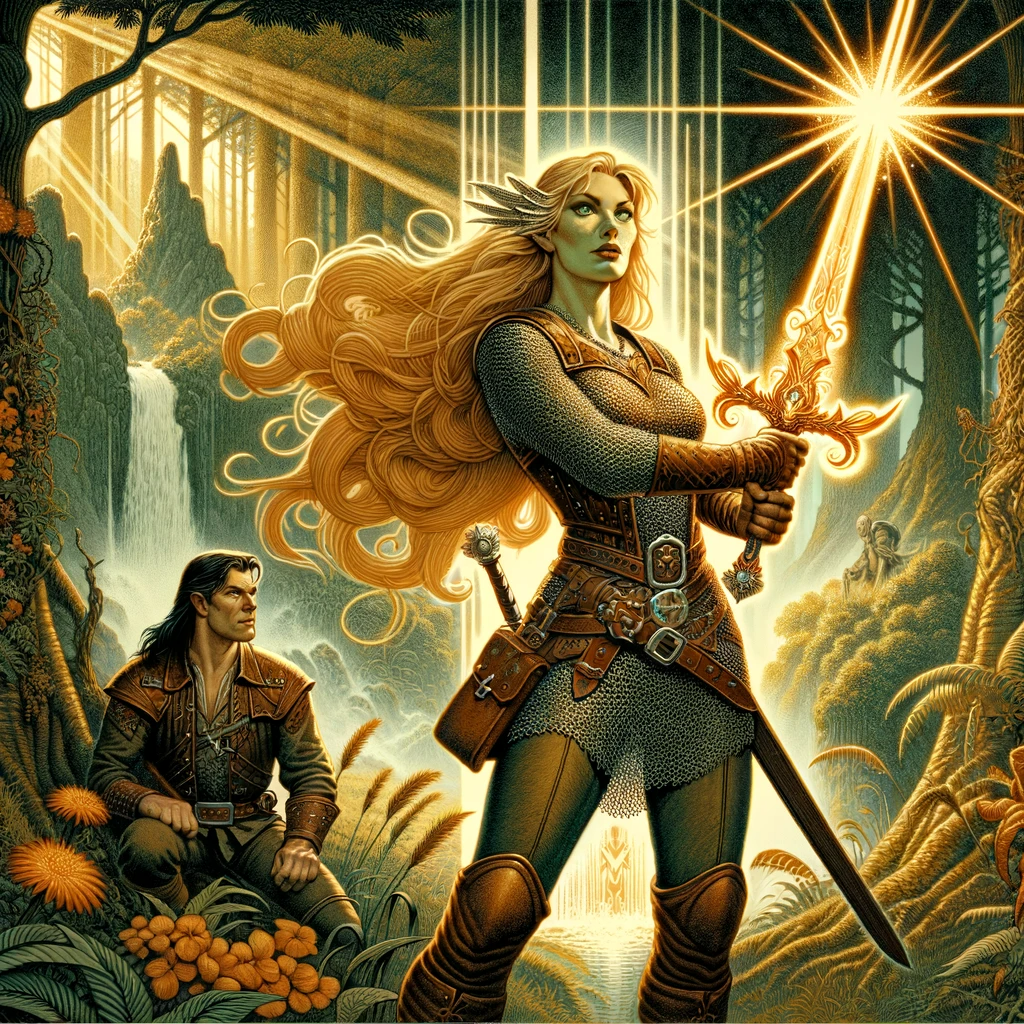
\includegraphics[width=0.5\textwidth]{brightblade.png}}~\\[1cm]
Brightblade
}
\addcontentsline{toc}{part}{Brightblade}

\chapter{Adventurers}
The world of Mundthir is a boon for some, a curse for others; but I'd say it's best for none other than the adventurer. 

Yes, the adventurer! That plucky man or woman, who travels Mundthir and its vast continents, and kingdoms that sit upon it, in order to seek fortune, fame and all of that vapourous gubbins.

I don't mean to fully put down the oh so humble adventurer. There have been many occasions where the noblest amongst them have used their skills and sometimes even their life to save Mundthir from dark threats. What's more if I was to put down adventurers as a whole, I would certainly be putting down myself!

Aye reader, that's right. I was an adventurer starting near one-hundred and thirty two years ago, only truly stopping in the last decade or two. It's been a long and interesting life all told, with many an adventure to call my own, with many a dear friend to share them with. Even so (and most half elves my age wouldn't like to admit it) our fey blood doesn't stop this feeling of thinness in your soul, like you've cheated the reaper decade after decade. I'm sure after all I've been through he'll have some choice words for me.

I apologise dear reader. Adventurers. They used to be a copper piece in a dragons horde. Common as muck. And there was good reason for it; all across Mundthir, there's ageless bounty to be found for those with a death wish to look for it. 

Case in point, I once knew an adventurer named Trimst. She was a lovely barbarian lady from the Gorthian Steppes, some north east way of Noth. Being in so close proximity to that intolerable and black kingdom she rode east near Priaethier, a small republic that unfortunately doesn't exist any more, but where I was adventuring myself at the time, in order to find a weapon that would be able to defend her people.

She knew of the Brightblade. A weapon of shimmering gold, and a magical heat that was of legend. The same legends said it was the property of the old emperor of Tet-Tehtu, a almost obscure figure from an obscure empire by the time of writing; but such legends passed by oral and musical tradition in Gorthia kept the knowledge alive in ways our written southern tradition could not. It's funny how that tends to be the case.

We'd met in a Priaethierin tavern in the capital, the Lost Dog. I'd travelled to Ars Priaethier after taking my leave from some small incident which \textit{I will not} go into, and she'd been the first thing that had caught my eye. Not to toot her horn too much, that is to say; the denizens of the Lost Dog looked hapless and forlorn to be sure; but she still stood out like a flame in the dark.

Trimst was muscular, pretty, and bubbly; with bouncing blonde hair that swept around as quickly as her eyes did. And that's what drew me to her ultimately, her eyes; for if she didn't have those wary, suspicious eyes so characteristic of someone who's fought many battles, then I'd have just written her off as some runaway.

So we sat and chatted, and much a credit to her Gorthian heritage she boasted of past fights, and past drinks. As we had tankard of ale after ale the stories turned to legends, and legends to songs, and songs to simply waving her sword around challenging any fool to a fight. Thankfully there were no fools to be found, and so no fight to be had, a fact that genuinely saddened her.

When the mood died, she told me of her quest, and how she'd come to know of it. That she was to look for the Tet-Tehtan tomb of the old emperor. I knew a little of that old culture though, and their habit of using traps. I warned her that I was seeking gold in a Tet-Tehtan crypt a decade ago, and that the dangers posed were not that of any simple dungeon to be raided.

But she laughed her iconic throaty laugh, almost as if putting on for a show, and told me, ``Aye, but caution is for those who plan to grow old my friend. I plan to live forever through legend and song!''

As I wrote before dear reader... a death wish. 

But so enraptured by her spirit and finding common cause with our hatred of the kingdom of Noth, we decided to band together. I rationalised it by thinking that I was stronger now, smarter, and a lot more careful. There was bound to be hoards of treasure in a Tet-Tehtan tomb, all of which would likely go to myself since Trimst only wanted the sword. 

We made plans as all good adventurers did. We agreed on a split to the loot (as I suspected all she wanted was the fame and the sword, which was fine by me), but then it dawned on me. Where were we to go? At the question Trimst took a deep drink on her ale, grinning like the drunk barbarian she was.

``I know exactly where we're going chum!'' She exclaimed. ``We're headed where the songs lead us!''

She got onto her stool, and wobbling she stood upright. Once she'd found her balance, she began singing;

%https://tex.stackexchange.com/questions/160560/package-to-typeset-poems

\begin{poem}
\begin{stanza}
``We wish you best in every age\verseline
We sing of clashes, slashes, steel\verseline
Warriors filled with mirth and zeal\verseline
Of tales of old, and fates ere sealed\verseline
But the greatest warrior who's love we feel;\verseline
That's our Friskr Brokensage!
\end{stanza}
\begin{stanza}
He travelled far and travelled south\verseline
Tuhtsin woods and further too\verseline
Where mountains travel two by two\verseline
And the river Ai-Crans flows through\verseline
To find the Valley of Tehtu\verseline
And to the river's mouth
\end{stanza}
\begin{stanza}
And there he found a castle dour\verseline
Of marble jewels and useless things\verseline
He ripped the draw bridge off its hinge\verseline
He climbed the rampart swift as wings\verseline
Drank and then began to sing\verseline
And drank more by the hour
\end{stanza}
\begin{stanza}
Friskr raided the castle larder\verseline
A warrior with eyes so cold\verseline
And wearing armour made of gold\verseline
`Screamed leave this place you upright gnoll!'\verseline
And struck our hero, a move too bold\verseline
So Friskr struck back harder!
\end{stanza}
\begin{stanza}
Then with every clash of sharpness made\verseline
Friskr's blade began to crack\verseline
`Sunder' his sword could not attack\verseline
Through the defence and the tact\verseline
`How can you beat me Tet-Tehtac?'\verseline
`You face the might of Brightblade!'
\end{stanza}
\begin{stanza}
Friskr fell back with a thud\verseline
Sunder cracked in twain\verseline
All he felt was pain\verseline
Nere was he seen again\verseline
But memories we retain\verseline
In our songs and Garthian blood!''
\end{stanza}
\end{poem}

I'd never heard the song before, but it wouldn't be the last time that I'd hear it. The legend of Friskr. My mind raced about the legend, picking up clues and directions to go in. The Ai-Crans did lay inbetween two mountain ranges somewhere south of Ars Priaethier. I also knew that this Tuhtsin woods was the old name for the woods of Praethierin. We could find this castle, which I guessed were likely ruins at that point, and nab Brightblade from a corpse, as well as the other jewels and trinkets left behind by this Friskr fellow.

It was foolish, I know. It seemed I had a death wish too. I'm sure Mr Reaper was tapping his foot impatiently as he saw the two of us exit the tavern to leave the city that very night. On our quest to find Brightblade.

\chapter{Interdiction}
We slept that night in the woods, having made blindly and drunkenly out of the city. I thank the Three every morn for the protection they gave to us; stumbling in the dark like idiots. I woke up under an old pine, covered in its leaves and the morning dew. Wiping my face and sitting up, Trimst lay in the middle of the clearing we stopped at, illuminated by the morning sun as if by limelight in a play.

Spread like a starfish and flat on her back, she snored loudly. That was something I'd come to know in the following days. And not just her snoring, but she did everything loudly; boasted the loudest, sang the loudest, couldn't even sneak past a drunken dwarf, especially in the chain-mail she loved to wear at all times.

Seeing as I was first up, I decided to take inventory. My rations, a bedroll (which I really should have used), some good strong elven rope from Llandwyllen, a deep-dish cast iron pan and a small purse of coin, which I kept for emergencies. It'd been too many times before that I had lost my coin purse to some pickpocket in Ars Priaethier.

I checked my belt and there it was, never having left my side. Gwythenril, my steel sword. I pulled it out of the scabbard and held it to the light, something I was fond of. It shimmered in hues of silver and blue.

However, pulling Gwynthenril out of his home, made a loud scratching sound, awakening Trimst. With a loud exagerrated yawn, very alike to roar, she sat up and stretched, the dew and chainmail glistening in the early rays.

``Ah my good friend!'' she boomed, noticing me for the first time. ``Have we any breakfast this morn?''

``Have you no rations of your own?'' I asked. It wasn't until then that I realised that she had no backpack, no rations, no provisions of any kind, aside for the armour she wore and the sword she kept.

``Raaa-shuns?'' Trimst mouthed the words as if she was hearing them for the first time, and thinking back it might have bloody well been her first time. ``I've nary any of that. Does it taste good? Was it a good kill to hunt?''

I chuckled to myself and pulled out a box of smoked sausages, mushrooms, dried bread, and cheese. Everything necessary to have a good breakfast on the road. ``We can do a bit of hunting later I think.'' I murmered taking out my cast iron pan and arranging some nearby twigs and rocks into something approximating a fire.

``Friend, those are way too wet for a fire!'' Trimst chuckled. ``Are you sure you've done this before?''

``Sure I have.'' I retorted, whipping her an annoyed glance. I twisted my hand into a magic sign; my index finger over my middle, and my ring finger turned 90 degrees straight, the sign of flame; and then speaking the magic words ``Yiklorkakis'' the wet leaves and branches dried instantly, sparked, and caught on fire.

To this Trimst eyes lit up, as she got to her feet hooting and hollering. ``That's absolutely amazing half elf! Do all of your kind know how to do that? I've nary seen any of the like!''

``Have you never met a half elf before?'' I asked Trimst, to which she shook her head.

``Never in my life. The fey folk don't especially travel up to Gorthia. I've always thought it was because of the lack of trees.''

``That is true, you hear of elves in the mountains and the trees; or in massive enclosed cities hidden by magic but truly never the steppes.'' I mused. ``Well my mother was a wood elf from-'' I cut myself short. I could hear rustling from some kind of creature from just outside the clearing. I had thought these parts were safe, but it was a rookie mistake to be so exposed and visible. Holding up my hand, Trimst instantly knew that something was wrong, and her ever watchful eyes focused upon the treeline.

Dark shapes, that's the first thing I saw, but Trimst saw something more. She screamed ``Watch out!'' before a searing pain shot into my back. I whipped around striking with Gwythenril into nothing but air.

``What is it? What did you see?'' I called to Trimst. But before she could answer there was another searing pain; this time in my leg. Looking down I could finally see what it was. An arrow, short and brutal sticking into my thigh. I could see the shooter in the treeline making for another shot, grinning with pointed teeth around fetid green skin. A goblin. With pointed ears and dark pupilles eyes, goblins are, dear reader, some of the most common of the evil fey that exist in the wild. They're not to be trifled with as their pack tactics can make a mincemeat of any adventurer. 

I could see that Trimst understood the situation before I could as she dashed past me, screaming with her sword in tow. Letting out a war cry she whipped her sword, expertly towards the goblin's head. But the sword found nothing but a nearby tree, as the goblin immediately dropped to his stomach, cackling at the folly of the barbarian.

He pulled out a nasty jagged dagger, and attempted to stick Trimst with it in the leg; but pulling away in time she brought her boot down on the goblin's head, bringing it firmly down into the dirt. When the goblin showed signs of squirming under her heel, she brought it up again and repeated the brutal attack. Again and again she stomped, until the bruised head of the goblin smashed like a melon, spewing black blood across the grass.

Unfased, she smiled at me and noticing the extra arrow in my leg asked, ``What's wrong half elf? Need help taking those arrows out?''

But I couldn't get the most important singular fact about goblins out of my head.

Goblins hunt in packs.

As soon as the thought crossed my mind, an explosion in the center of the clearing cracked, sending myself and Trimst to the floor.

Three more of the foul creatures emerged from the clearing; two running at us and the third, the leader of the bunch, sauntering out with a cocky self assured approximation of a smile. Unlike the others, his skin was pale. He wore robes with fingers, bones, ears, and all other manner of disgusting trophy tied to it with a piece of string. Holding a staff in one hand he pointed with the other, and gave directions to the two bandits in his guttural language. 

One set upon Trimst, but before I could get up to help her the other jumped onto my back, stabbing down with his knife. I spun around with force and speed, flicking the goblin off of my back, but leaving the knife buried in my shoulder plate. The goblin was on his feet though, and I realised too late that I did not get the goblin off my back due to any sort of combat skill, but rather because he wanted to jump off of my back. He wanted me to focus on him. 

Instinctively, I dove out of the way and my fears were confirmed, a bolt of magical water that would have struck me from behind sailed past me, and stuck the goblin right in his twisted and ugly maw. The pale goblin mage had done this, and I realised that they were better organised than I had thought. The mage must have held back at the last second, as the goblin in front of me was unharmed, save for him being soaked in water.

Save for him being soaked in water. 

He smirked at me, confident that the next magic bolt would end me, but I made the transmutation sign of fire and shouted the word ``Yiklorkakis!''. He dried up within the second, and burst into flame the next. The smell of roasted, rotten, meat and the screams of goblin curses filled the air as he ran wildly into the forest's edge. The feeling was so satisfying, and I chuckled to myself while scanning the rest of the clearing; looking for the pale mage, looking for Trimst.

I found Trimst first, she had gotten the better of her goblin foe; and with one smooth, practised motion, with enough speed and power to leave a crescent moon shaped after-image with her blade, she decapitated the goblin, sending the head flying into a nearby tree.

``Good'' I thought.

We both focused our gazes upon the final goblin, but he was already in the middle of weaving his next spell, murmuring the magic words. I shouted to Trimst ``Shut his mouth!'' and we both bolted for him, but before we could tackle the brute he disappeared. 

How a goblin knew that much magic, I could not say back then. I swore and helped Trimst up, suddenly feeling very weary over the whole ordeal.

We checked the bodies of the goblins that we'd slain, but could find no orders or indication as to their ultimate goal. I found a few extra gold pieces on one of them, which I passed into my coin pouch.

``What do you think they attacked us for?'' I asked Trimst.

She shrugged, beaming a wide smile with a touch of madness to it, and said ``It beats me. I'd never fought a goblin before though, it was pretty fun!''

I assure you she said those words, dear reader. Utterly hopeless. I decided to brush past it, saying ``We can reach the Ai-Crans within the day if we eat what's left of the breakfast and set off immediately. I'm sure that-'' but I cut myself short. The world around me was fading into a blackness from behind my eyeballs. Before I hit the floor I could hear Trimst asking if I was well, but I could not respond.

I thought that Mr Reaper finally was fed up with me. Maybe it would have been better if he was.

\chapter{Skald}
I awoke when the light of a sunbeam hit my face and a song of robins filled my ears. I was in a bed, cosy and rustic in appearance, with knitted covers and a wooden frame. The smell of bacon and other fried things filled my nostrils, and despite the sharp pain that racked my entire body I felt at complete peace.

I was in a log cabin, 

Looking to my side I saw an elderly man, with a large frame and sunken, but wise eyes. He smiled at me and stroked his long grey beard, a habit of his as I'd come to know. He wore a medallion of small skulls upon grey robes, with each skull having prescious gems set within their temples and eye sockets. He smoked a pipe with a long curved shank that went from his mouth down to the level of his chest. Wielding the pipe expertly, he took a long drag and chuckled to himself, smoke billowing lazily out of the corners of his mouth.

``You're quite the tough one, you know that right half elf?'' he said, looking at me up and down. ``Your friend wouldn't let me go until I healed you. That's not something necessarily in my repertoire, so I placed you here for rest, with the hope that your fey heritage would stave off  the worst of your injuries. I hope we can keep that detail between us.''

``Of course.'' I made out meekly, still recovering from the effects of the blade. ``I thank you all the same, Mr...''

He sat and stroked his beard some more, and the top of that self same beard curled into a gentle smile. Eventually he responded, ``You may call me Gallanrey. I'm somewhat of a researcher looking into the ecology along the Ai-Crans.''

``I see, and I'm guessing that's how you found us.'' I wheezed out.

``You guess correctly, half elf. I was looking for mushrooms within the Priatherin to prove a hypothosis of mine, when I heard the commotion. Goblins... they're definitely resourceful.


\part*{
\setlength{\fboxsep}{3pt}%
\setlength{\fboxrule}{3pt}%
\fbox{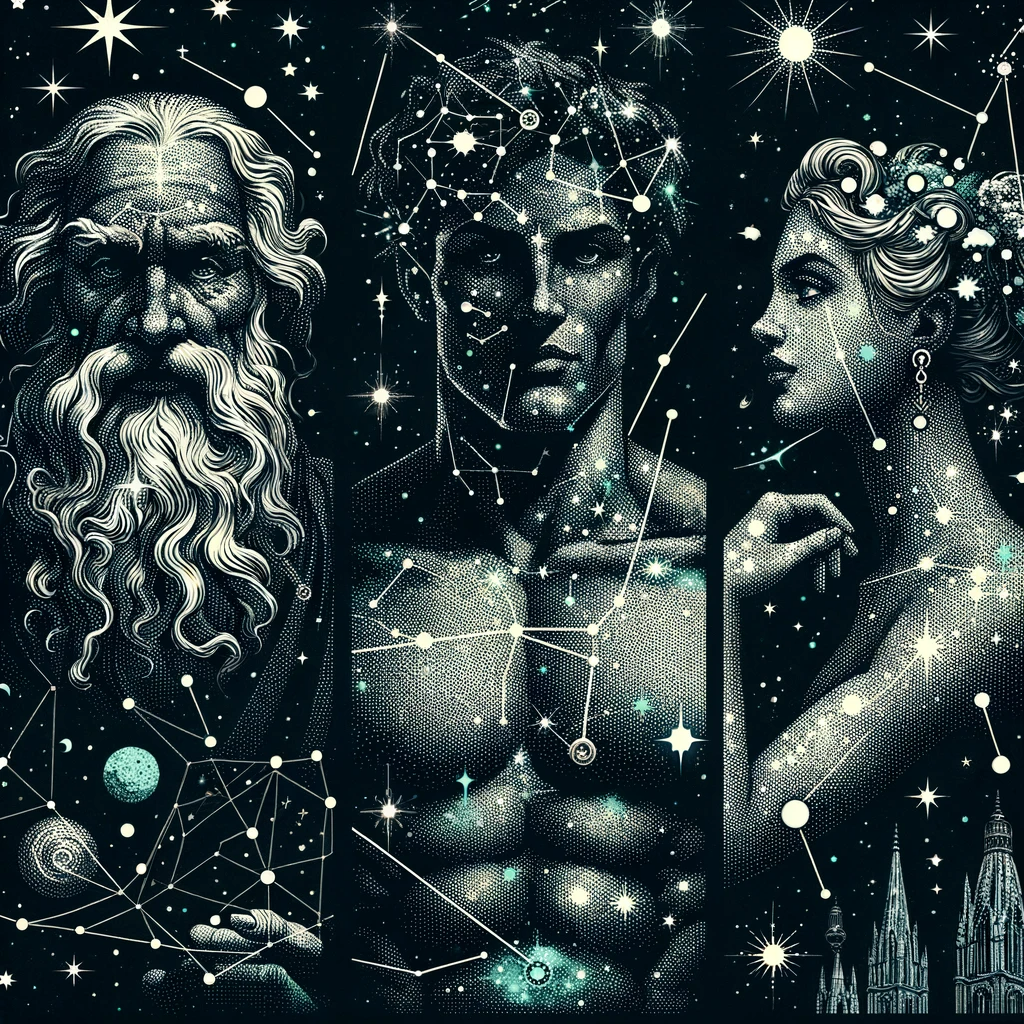
\includegraphics[width=0.5\textwidth]{the three.png}}~\\[1cm]
In Aeons Past
}
\addcontentsline{toc}{part}{In Aeons Past}
\setcounter{chapter}{0}

\chapter{Creation}
There was never a beginning to the universe, because that would mean there was a time before the gods. Amlaethon, Opferon and Khiron, three beings of immense power that were synonymous with the universe itself. Amlaethon was body of the universe; the stars and nebulae, the many worlds, and the verdant forests that grew upon them. Opferon was the motion of the universe; for when stars burned, celestial bodies crashed, rivers flowed, and trees swayed, it was opferon that made them do so. Khiron was the spirit of the universe; and he plotted each passing millenia, guiding the universe along its endless and infinite journey.

After the passing of countless Aeons, the gods grew dissatisfied with the perfect passing of the universe. All moved in accordance with their vision, and so all in the universe bored them. No longer was it enough to enjoy the plesentries of the life they'd created, and all the beauty that came with it, but they were to create a new type of life, one that was not under their constant care and control.

They named this life mortality, and they each passed their sublime being into the being of mortality to grow their creation.

Amlaethon gave mortality its body, mishapen and imperfect, the mortal was created without Khiron's guidance. Opferon 

\end{document}